\lecture{7}{17. Februar 2025}{Mechanical Properties, pt. 2: Plasticity}

\exercise{6.17} A cylindrical specimen of stainless steel having a diameter of \qty{12,8}{mm} and a gauge length of \qty{50,800}{mm} is pulled in tension. Use the load-elongation characteristics shown in the following table (\autoref{fig:f7_1}) to complete parts (a) through (f).

\begin{figure} [ht]
  \centering
  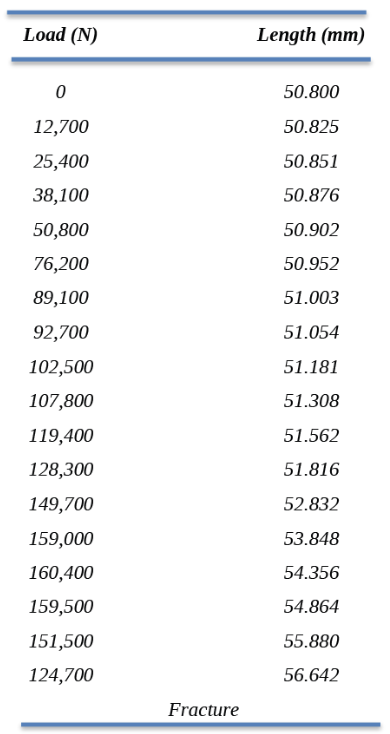
\includegraphics[width=0.35\linewidth]{./figures/f7_1.png}
  \label{fig:f7_1}
\end{figure}

\paragraph{(a)} Plot the data as engineering stress versus engineering strain.
\bigbreak
Engineering stress $\sigma$ can be found as
\[ 
  \sigma = \frac{F}{A} = \frac{\text{Load}\,(N)}{\pi \cdot \left( \frac{\qty{12,8}{mm}}{2} \right)^2} = \frac{\text{Load}\, (N)}{\pi \cdot (\qty{6,4}{mm})^2}
\]
whereas the engineering strain $\epsilon$ can be found as
\[ 
\epsilon = \frac{d}{l_0}
.\]
We can plot these two quantities as:
\begin{figure} [ht]
  \centering
  \caption{Plot of stress vs. strain for the given data points}
  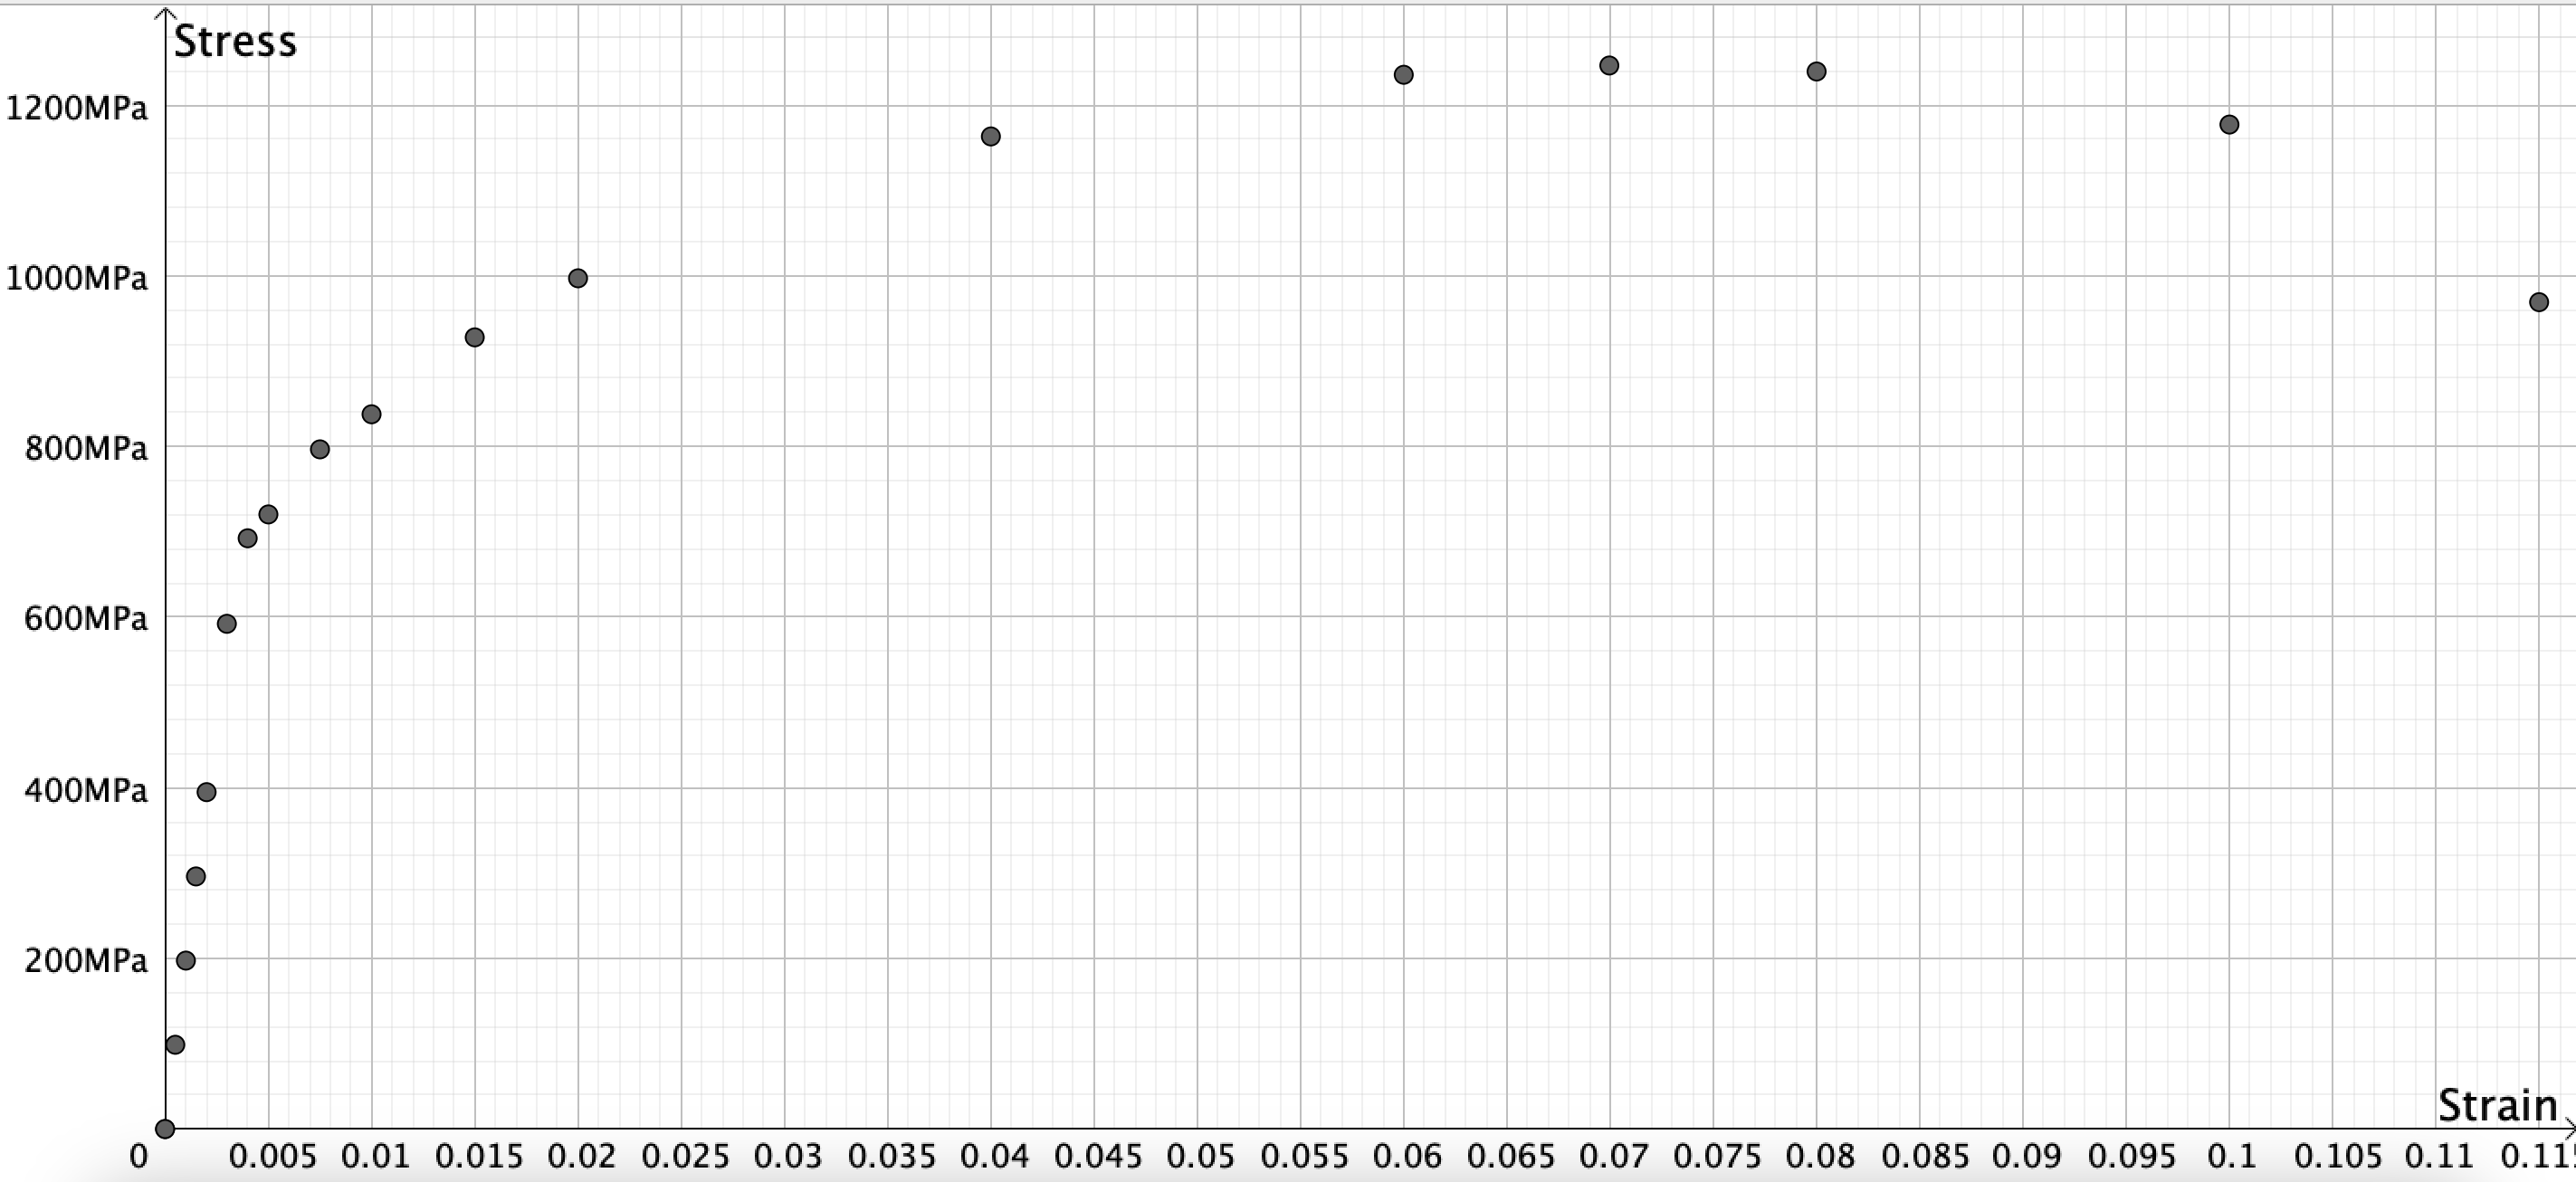
\includegraphics[width=0.8\linewidth]{./figures/f7_2.png}
  \label{fig:f7_2}
\end{figure}

\paragraph{(b)} Compute the modulus of elasticity
\bigbreak
The modulus of elasticity is approximately equal to the slope of the linear part at the start of the graph (the elastic region). To calculate the modulus of elasticity we will therefore just fit the first few points to a line. If we try to use 7 points we get a linear fit with $r^2 = \num{0,98976}$ but it becomes clear the 7th datapoint already is not quite linear. Therefore we try the first 6 which gives $r^2 = \num{0,99996}$. This gives a Young's modulus of $E = \qty{197,493}{GPa}$ as shown in \textbf{\autoref{fig:f7_3}} where a linear fit has been made on the first points in \textbf{\autoref{fig:f7_2}}.

\begin{figure} [ht]
  \centering
  \caption{Linear fit of the first 6 data points}
  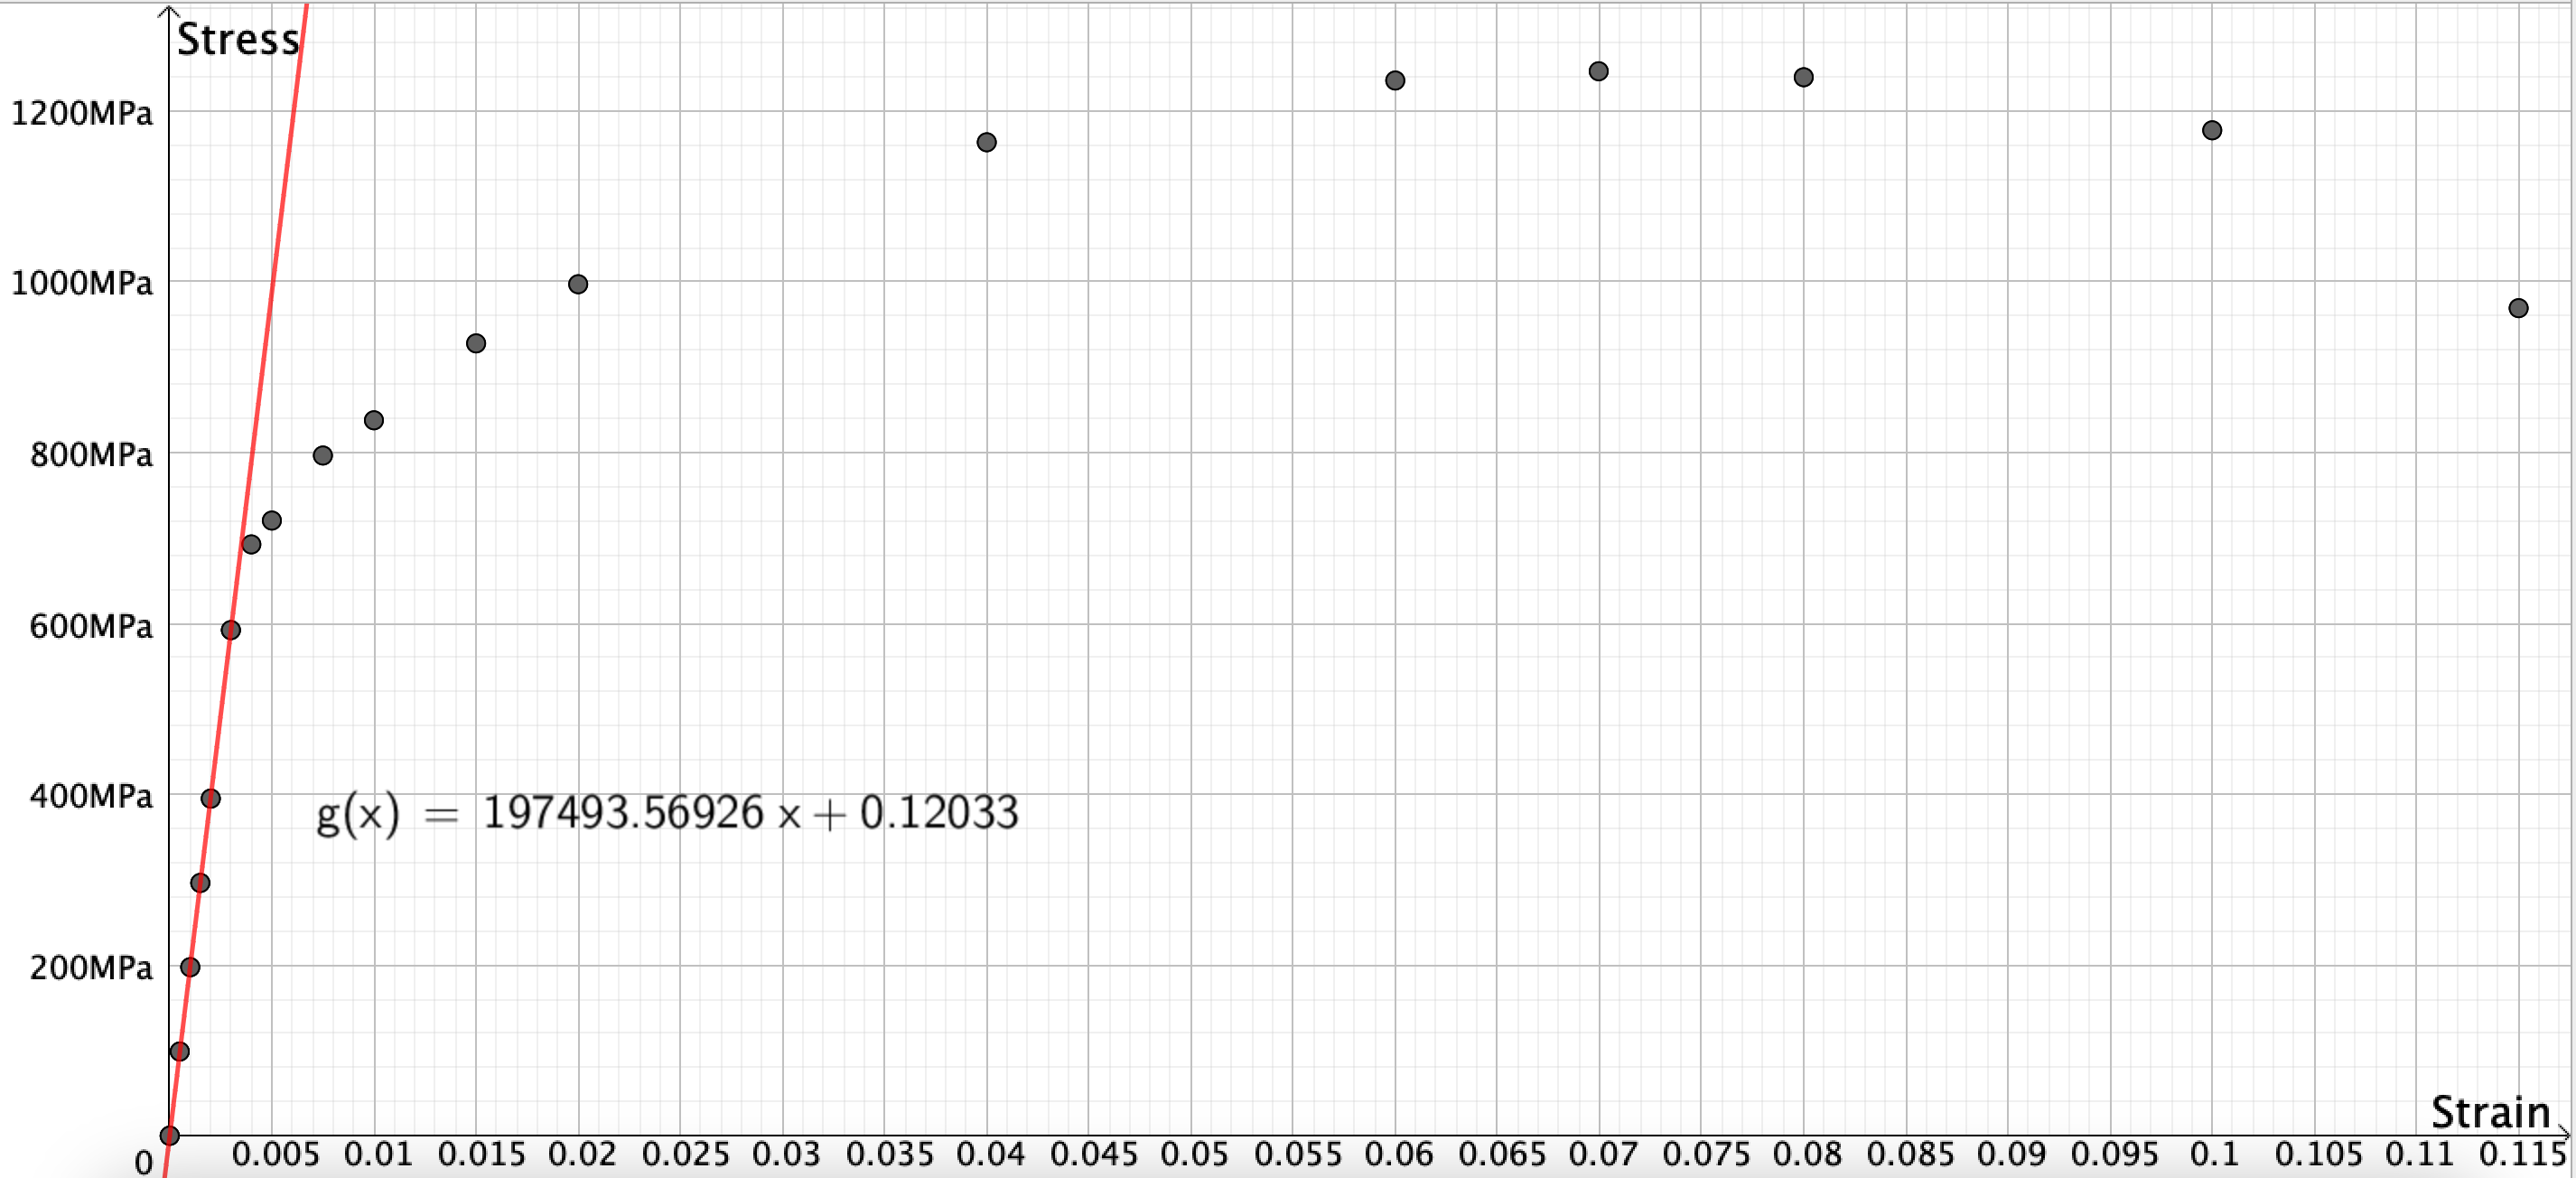
\includegraphics[width=0.8\linewidth]{./figures/f7_3.png}
  \label{fig:f7_3}
\end{figure}

\paragraph{(c)} Determine the yield strength at a strain offset of \num{0,002}.
\bigbreak
By constructing a straight line with the same slope as the linear fit on \textbf{\autoref{fig:f7_3}} and an $x$-intercept of $\epsilon = \num{0,002}$ we can determine the yield strength of the metal by finding the intercept between this line and the stress-strain curve. To appoximate the stress-strain curve we use linear interpolation as shown in \textbf{\autoref{fig:f7_4}}.
\begin{figure} [ht]
  \centering
  \caption{Linear interpolation to find the yield strength}
  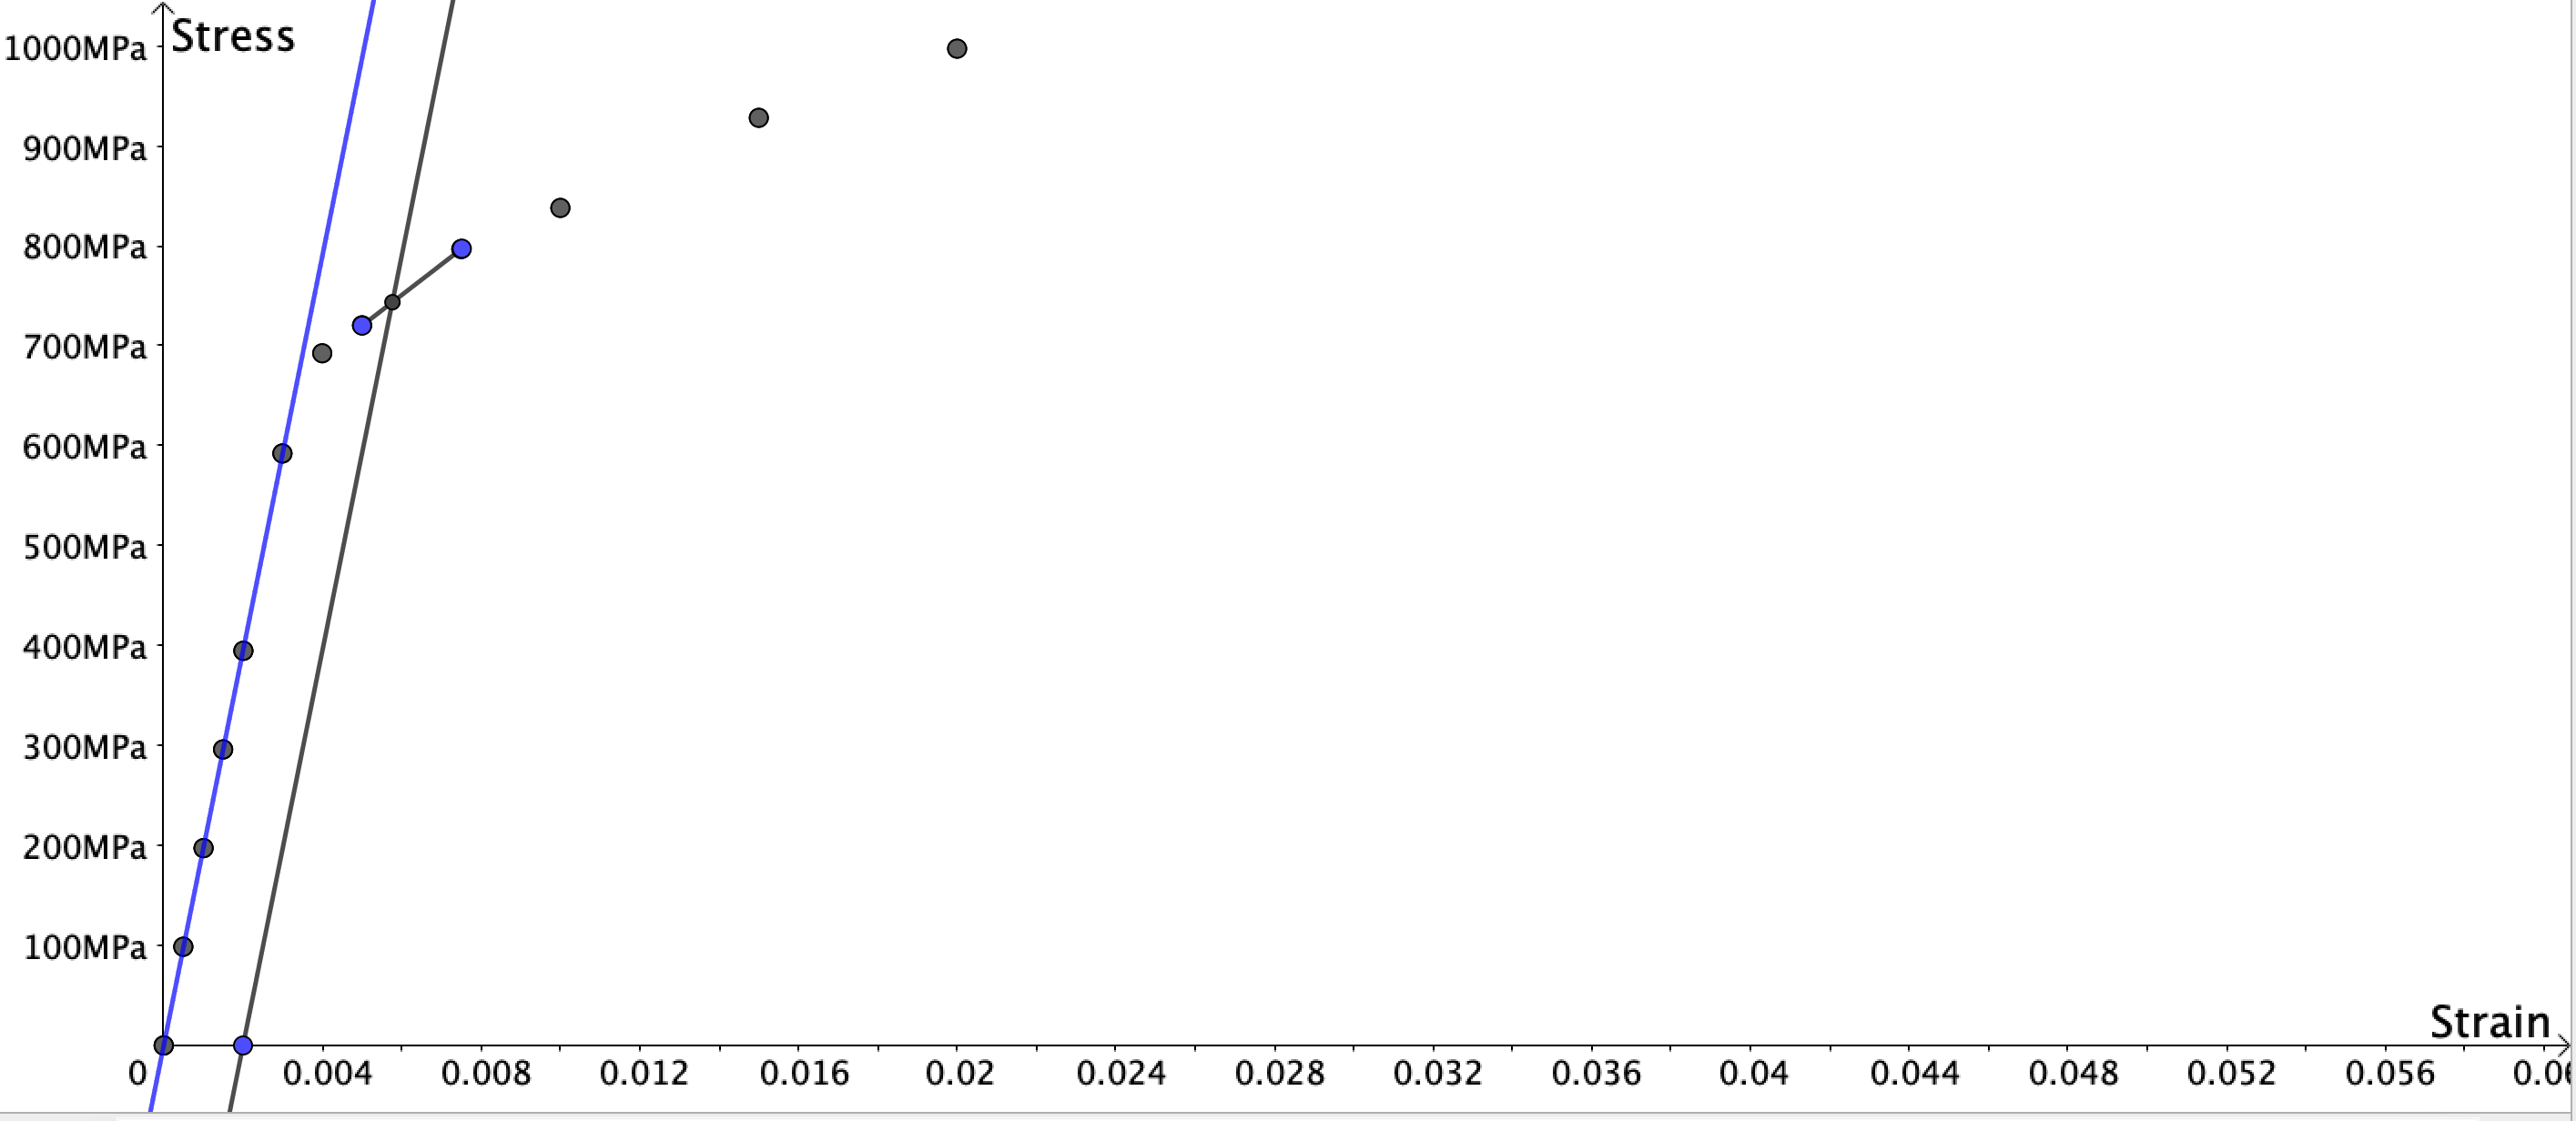
\includegraphics[width=0.8\linewidth]{./figures/f7_4.png}
  \label{fig:f7_4}
\end{figure}
From the above it can be seen that $\sigma_y = \qty{743,4}{MPa}$.

\paragraph{(d)} Determine the tensile strength of this alloy.
\bigbreak
The tensile strength $\sigma_{\mathrm{TS}}$ is simply the maximum amount of stress on the stress-strain curve. In this case we do not have a curve but only individual points. One could try to fit a function to the data, but as the three points with the highest stress look to be almost linear it is a reasonable approximation just to set $\sigma_{\mathrm{TS}}$ as the maximum stress in the dataset, as $\sigma_{\mathrm{TS}} \approx \qty{1246}{MPa}$.

\paragraph{(e)} What is the approximate ductility, in percent elongation?
\bigbreak
The ductility in percent elongation can be found with the formula
\[ 
  \% \mathrm{EL} = \frac{L_f - L_0}{L_0}
.\]
Where $L_f$ and $L_0$ is the length of the specimen after and before loading. By substituting in known values we get
\[ 
\% \mathrm{EL} = \frac{\qty{56,642}{mm} - \qty{50,800}{mm}}{\qty{50,800}{mm}} \approx \num{11,5} \% 
.\]


\paragraph{(f)} Compute the modulus of resilience.
\bigbreak
The modulus of resilience is given by
\[ 
U_r = \frac{\sigma_y^2}{2E}
.\]
By substituting in known values we get
\[ 
U_r = \frac{(\qty{743,4}{MPa})^2}{2\cdot \qty{197,493}{GPa}} = \qty{1,3991}{MPa} = \qty{1,3991}{\frac{MJ}{m^3}} 
.\]


\exercise{6.29}

\paragraph{(a)} What is the indentation diagonal length when a load of \qty{0,60}{kg} produces a Vickers $\mathrm{HV}$ of \num{400}?
\bigbreak
Vickers $\mathrm{HV}$ is given by
\[ 
\mathrm{HV} = \num{1,854} \frac{P}{d_1^2}
\]
for a load $P$ in \unit{kgf} and a length of the diagonal $d_1^2$ given in \unit{mm}. We solve the above equation for $d_1$ as
\[ 
d_1 = \sqrt{\frac{\num{1,854} P}{\mathrm{HV}}} = \sqrt{\frac{\num{1,854} \cdot \qty{0,6}{kgf}}{\qty{400}{\frac{kgf}{mm^2}}}} = \qty{0,0527}{mm}
.\]


\paragraph{(b)} Calculate the Vickers hardness when a \qty{700}{g} load yields an indentation diagonal length of \qty{0,050}{mm}.
\bigbreak
We can reuse the above formula for the Vickers $\mathrm{HV}$ as
\[ 
\mathrm{HV} = \num{1,854} \cdot \frac{\qty{700}{g}}{(\qty{0,050}{mm})^2} = \qty{520}{\frac{kgf}{mm^2}} 
.\]

